% !TEX root = ../Slides-IntroPythonJupyter.tex
\frame{\frametitle{Python}
\begin{columns}[t] 
     \begin{column}[T]{7cm} 
     	\begin{itemize}
		\item Interpreted high-level language
		\item Focus on readibility
		\item Program structure by indentation - no braces
		\item Dynamically typed - no variable definition required
		\item Highly popular
		\begin{itemize}
			\item Provides numerous powerful packages
			\item Trained staff and freelancers available
		\end{itemize}
     	\end{itemize}
     \end{column}
     	\begin{column}[T]{7cm} 
         	\begin{center}
            		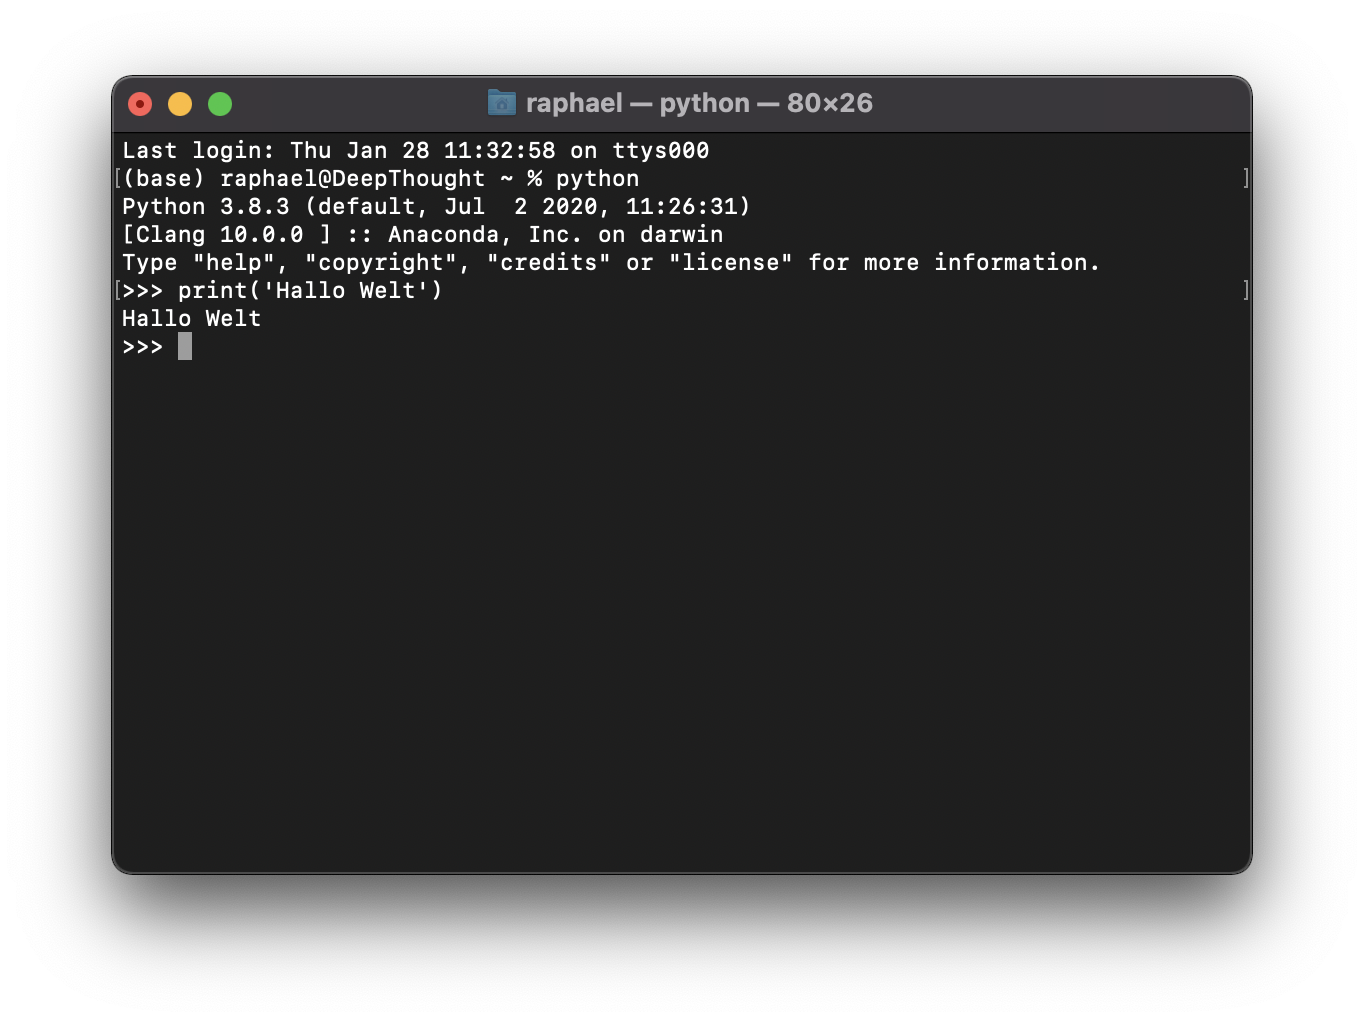
\includegraphics[width=0.95\textwidth]{TerminalHalloWelt}\source{}\\
		Python in Terminal
        		\end{center}
     \end{column}
 \end{columns}
}

\frame{\frametitle{Jupyter}
\begin{columns}[t] 
     \begin{column}[T]{7cm} 
     	\begin{itemize}
		\item Interactive Notebook
		\item Can contain Text, images, code
		\begin{itemize}
			\item Multiple languages, e.g. R, Julia, Python
		\end{itemize}
		\item Powerful combination of code, results and explanations - in one document
		\item Notable extensions:
		\begin{itemize}
			\item JupyterHub: Multi-User server
			\item JupyterLab: Enriched user interface, more formatting options
		\end{itemize}

     	\end{itemize}
     \end{column}
     	\begin{column}[T]{7cm} 
         	\begin{center}
            		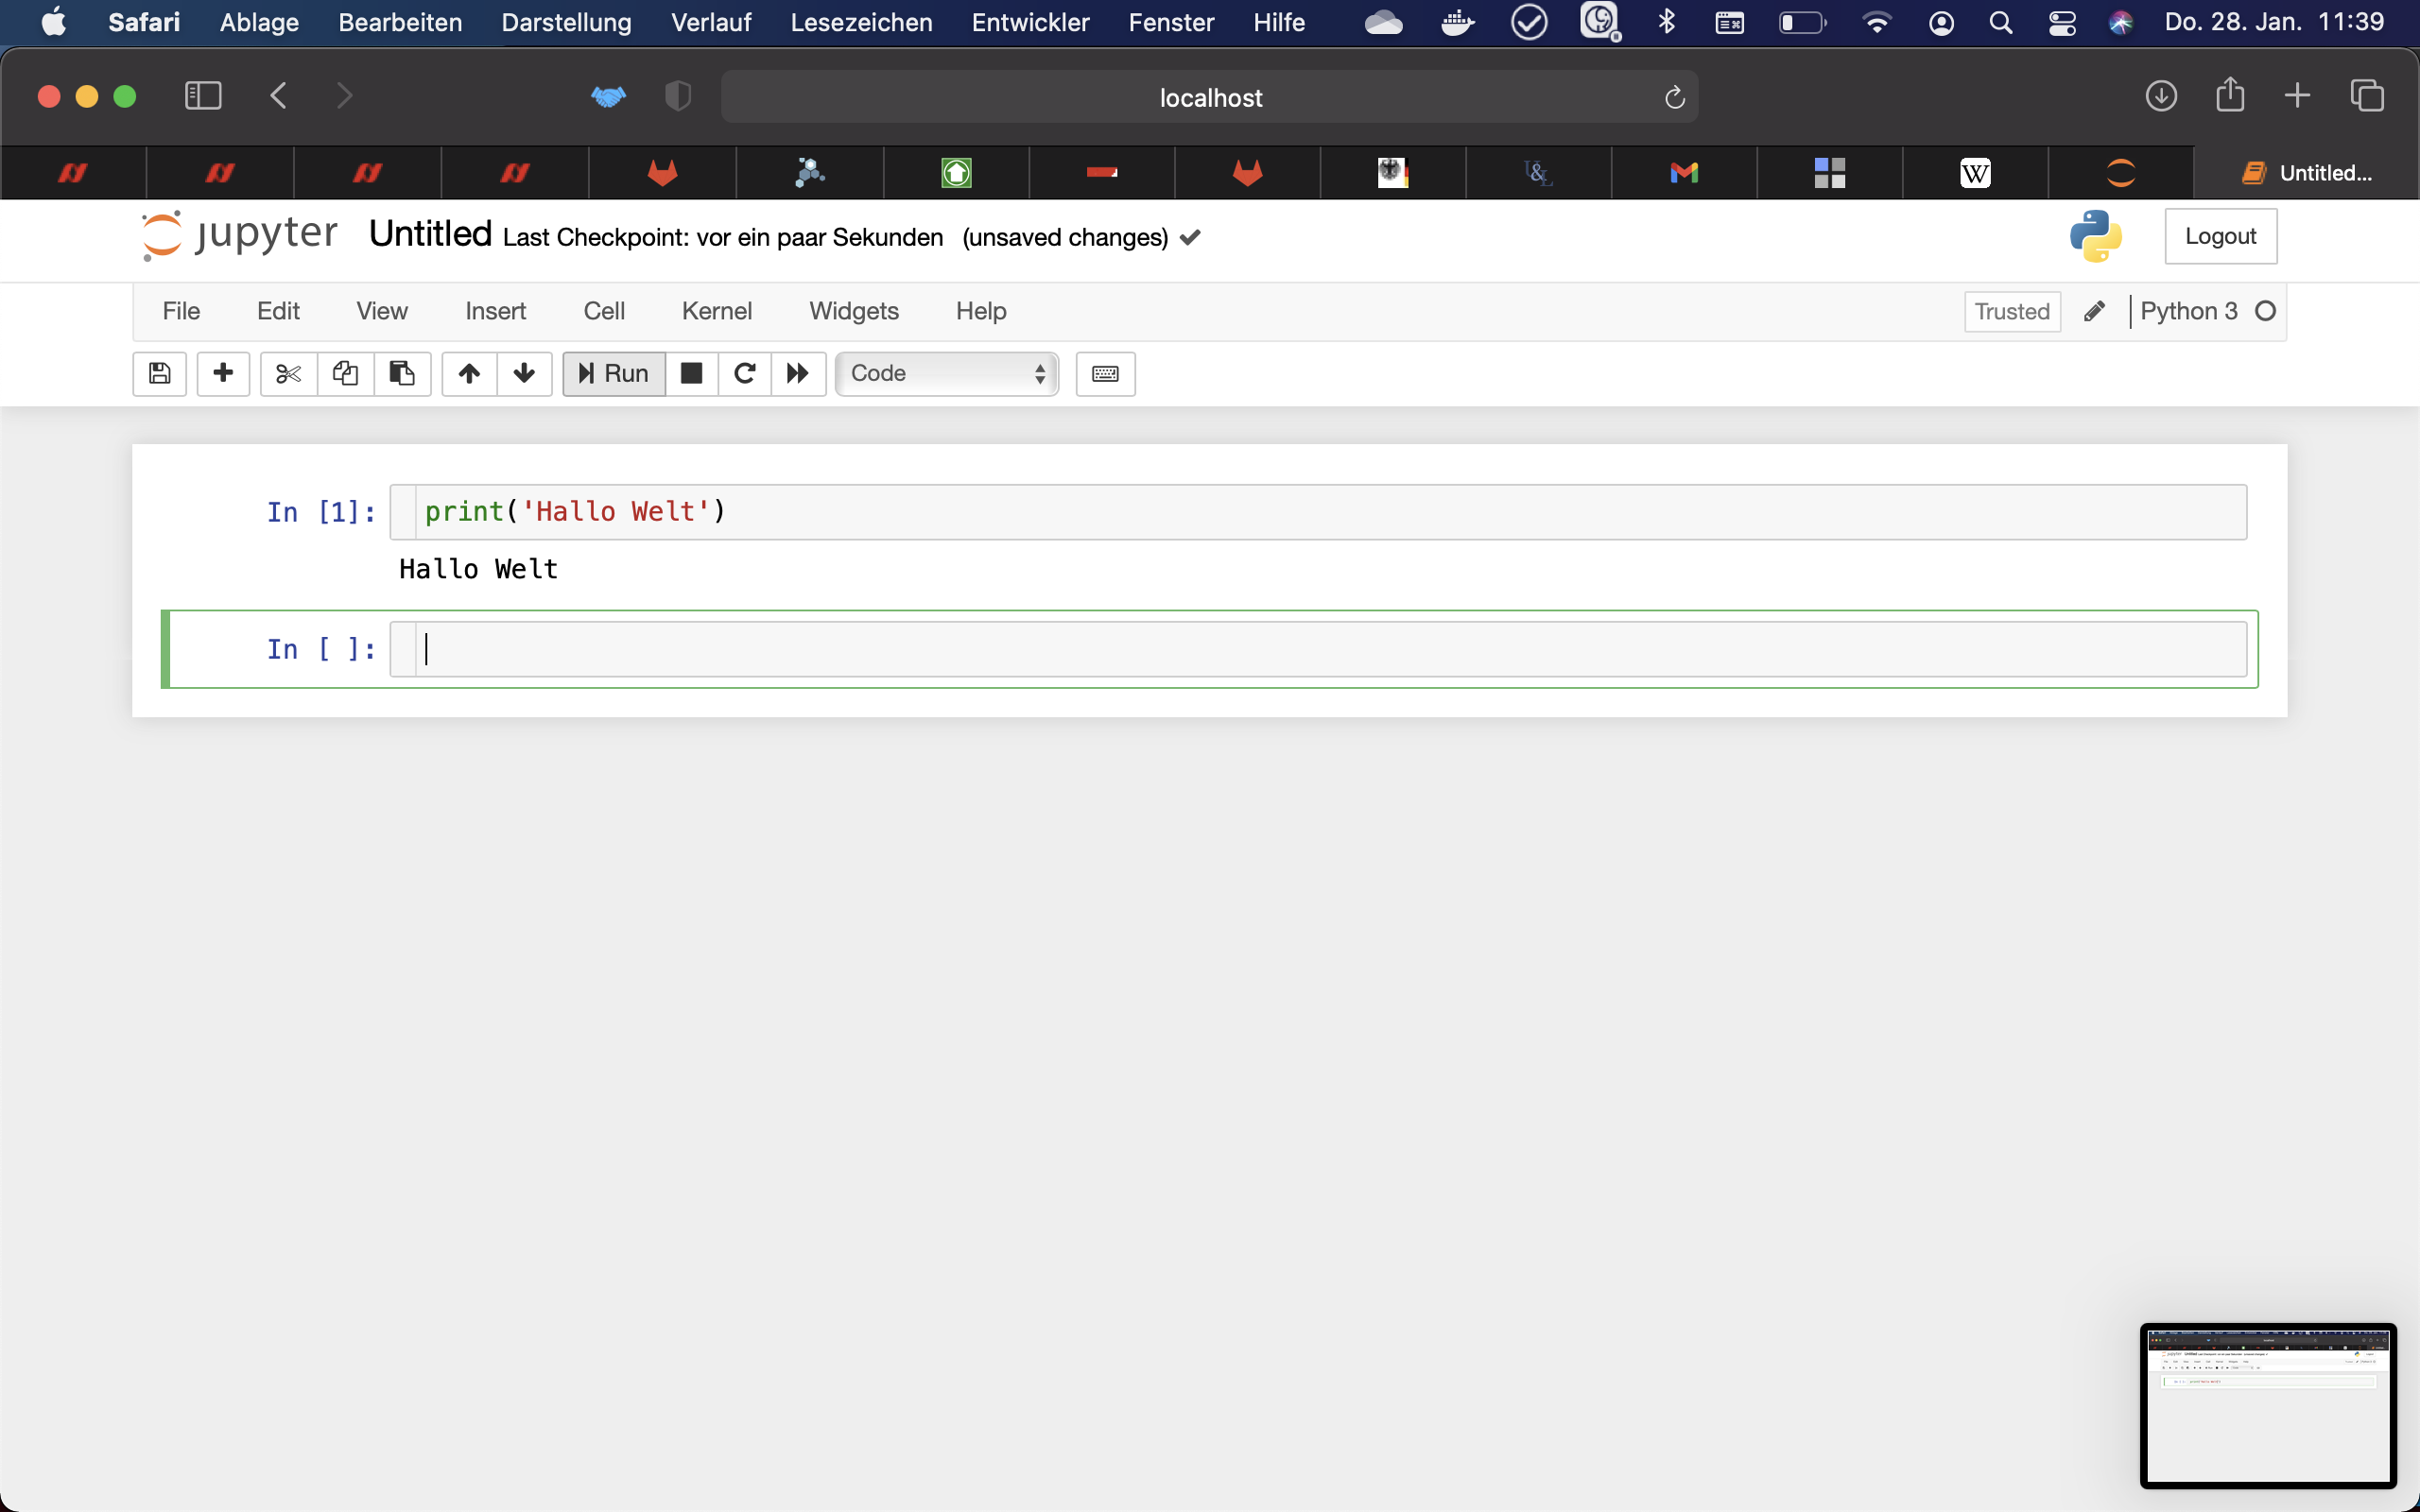
\includegraphics[width=0.95\textwidth]{JupyterHalloWelt2}\source{}\\
			Basic Jupyter Notebook
        		\end{center}
     \end{column}
 \end{columns}
}


\frame{\frametitle{Installation}
     	\begin{itemize}
		\item (Mostly) required: Anaconda\footnote{In case an installation is impossible, google Colab or Binder online-Solutions can be arranged.}
		\begin{itemize}
			\item Preselected python packages for data analysis 
			\item Package manager \texttt{conda}: conveniently add packages from console
			\item Environment manager
			\item Download at \url{https://www.anaconda.com/products/individual}
			\item Follow installation instruction
			\end{itemize}
		\item Convenient: Github desktop app
		\begin{itemize}
			\item Version control of code
			\item Clone course repository (and others...)
			\item Download at \url{https://desktop.github.com}{https://desktop.github.com}
			\item Follow installation instruction
		\end{itemize}
     	\end{itemize}
   }


\frame{\frametitle{Special packages individual branches}
     	\begin{itemize}
		\item Base packages: anaconda
		\item Using \texttt{conda package manager}
		\item Data analysis:
		\begin{itemize}
			\item Plotly: \texttt{conda install -c conda-forge plotly}
		\end{itemize}
		\item Simulation:
		\begin{itemize}
			\item PyControl: \texttt{conda install -c conda-forge control}
		\end{itemize}
		\item Computer Vision:
		\begin{itemize}
			\item OpenCV: \texttt{pip install opencv-python}
			\item Tesseract: \texttt{pip install tesseract pytesseract}
		\end{itemize}

     	\end{itemize}
   }



%
%\frame{\frametitle{Get started}
%\framesubtitle{Create your first jupyter notebook}
%\begin{columns}[t] 
%     \begin{column}[T]{7cm} 
%     	\begin{itemize}
%		\item Python 
%		\begin{itemize}
%			\item is interpreted
%			\item can be run on terminal or IDE
%		\end{itemize}
%		\item Indentation is strict, defines program structures (no braces)
%		\item Dynamically typed
%		\begin{itemize}
%			\item No variable declaration required
%		\end{itemize}
%		\item Syntax
%		\begin{itemize}
%			\item Refer to example worksheets
%		\end{itemize}
%		\item Data structures
%		\begin{itemize}
%			\item List: \texttt{l = [1, 2, ``a'']}
%			\item Tuples: \texttt{t = (1, 2, ``a'')}
%			\item Dictionaries: \texttt{d = \{``a'':1, ``b'':2\}}
%			\item Sets: \texttt{s = set(\[1, 2, 3, 4\])}
%		\end{itemize}
%	\end{itemize}
%     \end{column}
%     	\begin{column}[T]{7cm} 
%         	%\begin{center}
%            		\StickyNote[5cm]{
%			\begin{itemize}
%				\item[$\square$] Open a new jupyter notebook
%				\item[$\square$] Print ``Hello World''
%				\item[$\square$] Run a \texttt{for}-loop
%				\begin{itemize}
%					\item using \texttt{range(...)}
%					\item printing the loop variable
%				\end{itemize}
%				\item[$\square$] Create an example of the data structures listed
%				\item[$\square$] Access their elements
%				\end{itemize}}
%        		%\end{center}
%     \end{column}
% \end{columns}
%}
